\documentclass[tikz,margin=2mm]{standalone}
\usetikzlibrary{positioning, arrows.meta}
\usepackage{bm}

\begin{document}

    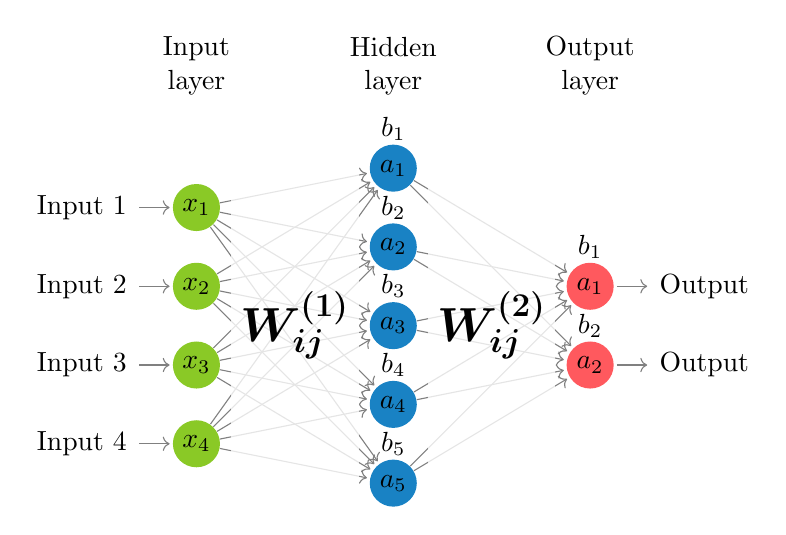
\begin{tikzpicture}[shorten >=1pt,->,draw=black!50, node distance=\layersep]
        \definecolor{inp}{HTML}{8ac926}
        \definecolor{hid}{HTML}{1982c4}
        \definecolor{outp}{HTML}{ff595e}
        \newcommand{\layersep}{2.5cm}
        \tikzstyle{every pin edge}=[<-,shorten <=1pt]
        \tikzstyle{neuron}=[circle,fill=black!25,minimum size=17pt,inner sep=0pt]
        \tikzstyle{input neuron}=[neuron, fill=inp];
        \tikzstyle{output neuron}=[neuron, fill=outp];
        \tikzstyle{hidden neuron}=[neuron, fill=hid];
        \tikzstyle{annot} = [text width=4em, text centered]

        % Draw the input layer nodes
        \foreach \name / \y in {1,...,4}
        \node[input neuron, pin=left:Input \y] (I-\name) at (0,-\y) {$x_{\y}$};

        % Draw the hidden layer nodes
        \foreach \name / \y in {1,...,5}
        \path[yshift=0.5cm]
        node[hidden neuron] (H-\name) at (\layersep,-\y cm) {$a_\y$}
        node[annot,above of=H-\name, node distance=0.5cm] (hl) {$b_\y$};

        % Draw the output layer node
        \foreach \name / \y in {1,2}
        \path[yshift=-1cm]
        node[output neuron,pin={[pin edge={->}]right:Output}] (O-\name) at (2*\layersep,-\y) {$a_\y$}
        node[annot,above of=O-\name, node distance=0.5cm] (hl) {$b_\y$};

        % Connect every node in the input layer with every node in the
        % hidden layer.
        \foreach \source in {1,...,4}
        \foreach \dest in {1,...,5}
        \path (I-\source) edge (H-\dest);

        % Connect every node in the hidden layer with the output layer
        \foreach \source in {1,...,5}
        \foreach \dest in {1,2}
        \path (H-\source) edge (O-\dest);

        % Draw a semi-transparent rectangular node with a bold "w" inside
        \node[fill=white!50, opacity=0.8, text opacity=1, font=\LARGE, minimum width=1.5cm, minimum height=4cm] at (0.5*\layersep, -2.5) {$\bm{W_{ij}^{(1)}}$};
        \node[fill=white!50, opacity=0.8, text opacity=1, font=\LARGE, minimum width=1.5cm, minimum height=4cm] at (1.5*\layersep, -2.5) {$\bm{W_{ij}^{(2)}}$};

        % Annotate the layers
        \node[annot,above of=H-1, node distance=1.3cm] (hl) {Hidden layer};
        \node[annot,left of=hl] {Input layer};
        \node[annot,right of=hl] {Output layer};
    \end{tikzpicture}

\end{document}